\documentclass[
    a4paper,
    11pt
]{article}

\usepackage[utf8]{inputenc}
\usepackage{float}
\usepackage{mathtools}
\usepackage{amssymb}
\usepackage{physics}
\usepackage{tabulary}
\usepackage{booktabs}
\usepackage{graphicx}
\usepackage{hyperref}

\author{Felix Köhler}
\title{Numerical Programming 1 (CSE @ TUM) cheat sheet}


\begin{document}

\maketitle

\tableofcontents

\clearpage

\section{General}

\subsection{Taylor Series}

One-dimensional Taylor-Series Expansion for a n+1 continously differentiable
function on the the interval a to b with a $\xi \in [x, x+h]$
\begin{equation}
    f(x+h) = \sum_k^n \frac{1}{k!} f^{(k)}(x)h^k + \frac{1}{(n+1)!}
    f^{(n+1)}(\xi)h^{n+1}
\end{equation}

\subsection{Euler's Formula}

\begin{equation}
    e^{ix} = \cos(x) + i\sin(x)
\end{equation}

\subsection{Trigonometric Identities}

\begin{equation}
    \sin(u \pm v) = \sin(u) \cos(v) \pm \cos(u) \sin(v)
\end{equation}

\begin{equation}
    \cos(u \pm v) = \cos(u) \cos(v) \mp \sin(u) \sin(v)
\end{equation}

\subsection{L'Hospital's Rule}

Technique to evaluate the limits of indertminate forms.

If $\lim_{x\to c} f(x) = \lim_{x\to c}g(x) = 0$ or $\pm \infty$ and $g'(x) \neq 0
\forall x \neq c$ then

\begin{equation}
    \lim_{x\to c} \frac{f(x)}{g(x)} = \lim_{x\to c} \frac{f'(x)}{g'(x)}
\end{equation}

Can be extended to higher order derivatives.

\subsection{Total Derivative}

First order
\begin{equation}
    \mathrm{d}f(x_1, x_2, ..., x_n) = \sum_{i=1}^n \pdv{f(\mathbf{x})}{x_i}
    \mathrm{d} x_i
\end{equation}

Second Order
\begin{equation}
    \mathrm{d}^2f = \mathrm{d}(\mathrm{d}f) = ... = \pdv[2]{f}{x} \mathrm{d}x^2 +
    2 \pdv[2]{f}{x}{y} \mathrm{d}x\mathrm{d}y + \pdv[2]{f}{y} \mathrm{d}y^2
\end{equation}

\subsection{Matrix Norms}

Adhere to the regular norm properties (greater than zero, homogenity, triangular
inequality)

\begin{equation}
    ||\mathbf{A}|| > 0, \quad \forall \mathbf{A} \neq \mathbf{0}, \quad
    (||\mathbf{A}|| = 0 <-> \mathbf{A} = \mathbf{0})
\end{equation}

\begin{equation}
    ||\alpha \mathbf{A}|| = |\alpha| ||\mathbf{A}||
\end{equation}

\begin{equation}
    ||\mathbf{A} + \mathbf{B}|| \leq ||\mathbf{A}|| + ||\mathbf{B}||
\end{equation}

Additionaly it can be \textit{sub-multiplicative}, if
\begin{equation}
    ||\mathbf{CD}|| \leq ||\mathbf{C}||\cdot ||\mathbf{D}||
\end{equation}

And \textit{compatible} or \textit{consistent} with a vector norm
\begin{equation}
    ||\mathbf{A} \vec{x}|| \leq ||\mathbf{A}|| ||\vec{x}||
\end{equation}

\subsection{Implicit Function Theorem}

States whether an implicitly given function $F(x, y) = 0$ can be expressed by an
explicit relation between its arguments $y = y(x)$.

In higher dimensions: Let $\vec{F}: U \times V \to \mathbb{R}^n, \quad U
\subseteq \mathbb{R}^m, \quad V \subseteq \mathbb{R}^n$.

In one dimensions with a two-dimensional input: Let $g(x, y) = 0$ be an
implicitly given function. Since $g$ is zero on the entire input set its (total)
derivative at every function point must also be zero. This can then be
rearranged to get the info of the derivative of the explicit functions with
respect to the other variable
\begin{equation}
    y^{'}(x, y) = - \frac{\pdv{g(x, y)}{x}}{\pdv{g(x, y)}{y}}, \quad
    x^{'}(x, y) = - \frac{\pdv{g(x, y)}{y}}{\pdv{g(x, y)}{x}}
\end{equation}
So at a given point $(x_0, y_0)$ that satisfies the implicit equation $g(x_0,
y_0)$ (use e.g. root finding methods to get such a value pair) we can also
easily get the values of the derivatives of $x$ and $y$. This can then be useful
to approximately rebuild the explicit function by the means of a Taylor
expansion.


\subsection{Gershgorin Disks}

Gershgorin disks give an estimate to where eigenvalues of a matrix lie in the
complex plain. Assume $A \in \mathbb{C}^{n x n}$
\begin{equation}
    R_i := \left\{z \in{} \mathbb{C} |
    |z - a_{ii}| \leq{} \sum_{\substack{j=1 \\ j\neq{} i}}^{n}|a_{ij}| \right\}
\end{equation}
The the set of z (=R) describe the Gershgorin disks in which the eigenvalue can
be found

\subsection{Matrix Properties}

\begin{itemize}
    \item Normal Matrices commute with their hermitian $\mathbf{AA}^T =
        \mathbf{A}^T \mathbf{A}$, every hermitian and every unitary matrix is
        normal
    \item Positive definite Matrices follow $\vec{x}^T \mathbf{A} \vec{x} > =0,
        \forall \vec{x} \in \mathbb{R}^n$
    \item Positive definite Matrix if hermitian follows Sylvester's Criterion:
        All the principal minors and the matrix itself must have a positive
        determinant
\end{itemize}

\subsection{Determinant of a square matrix}

\begin{equation}
    det(\mathbf{A}) := \sum_{j=1}^{n} (-1)^{j+1} a_{j1} det(\mathbf{A}_{j1})
\end{equation}

\subsection{Determinant of a block matrix by its blocks}

todo

\subsection{Taylor Expansion of Exponential Function}

Also valid matrix exponential

\begin{equation}
    e^z = \sum_{k=0}^{\infty} \frac{z^k}{k!}
\end{equation}

\subsection{Sum series}

Interrupted and to infinity geometric series

Leibniz-series error bound cut-off

Adam-Riese series

%%% ---------------------

\section{Polynomials}

\subsection{Monomial Basis}

\begin{equation}
    span\{1, x, x^2, x^3, ..., x^n\} = \Pi_n
\end{equation}

\subsection{Lagrange Polynomials}

On a set of points $t_i$ these polynomials are zero at $k \neq j$ and 1 at $k =
i$
\begin{equation}
    L_k(t) := \prod_{\substack{i=0 \\ i\neq j}}^{n} \frac{t - t_i}{t_k - t_i}
    \in \Pi_n
\end{equation}

\subsection{Chebychev Polynomials}

The Chebychev polynomials are directly defined by
\begin{equation}
    T_n(x) = \cos(n\arccos(x))
\end{equation}

Or by a three term recursion (it shares the first two polynomials with the
common monomial basis)
\begin{equation}
    T_n(x) = 2xT_{n-1}(x) - T_{n-2}(x), \quad T_0(x) = 1, \quad T_1(x) = x
\end{equation}

MinMax Property: Chebychev polynomials minize the $\infty$-norm (max-norm) on
the interval $x \in [-1, 1]$.

\subsection{Hermite Polynomials}

Require position and slope at each point. Can be used for Hermite cubic spline
interpolation, however then only $C^1$ over the nodes

\subsection{Legendre Polynomials}

The Legendre Polynomials form a basis of the space of polynomials and are
directly defined by
\begin{equation}
    P_n(x) = \frac{1}{2^n n!} \dv[n]{}{x}[(x^2 - 1)^n]
\end{equation}

The recursive definition is given by
\begin{equation}
    (n+1)P_{n+1}(x) = (2n+1)xP_n(x) - n P_{n-1}(x), \quad P_0 = 1, \quad P_1=x
\end{equation}

\subsection{Bernoulli Polynomials}

Form a basis of $\Pi_n$.
With $ b_0(x) := 1$ recursively defined as
\begin{equation}
    b_k'(x) = b_{k-1}(x) \quad \text{and} \quad \int_0^1 b_k(x) \, \mathrm{d}x = 0
\end{equation}

The first three read
\begin{equation}
    b_0(x) = 1, \quad b_1(x)=x - 1/2, \quad x^2/2 - x/2 + 1/12
\end{equation}

The integral fixes the integration constant.


%%% ----------------------------------

\section{Error Analysis}

\subsection{Condition Number}

General Relative condition nuumber for $\mathbf{f}:\mathbb{R}^n -> \mathbb{R}^m$ if the
peturbed input $\mathbf{\tilde{x}}$ approaches the non-perturbed
\begin{equation}
    \frac{||\mathbf{f}(\mathbf{x}) -
    \mathbf{f}(\mathbf{\tilde{x}})||}{||\mathbf{f}(\mathbf{x})||} \le
    \kappa_{rel}(\mathbf{f})(\mathbf{x}) \cdot
    \frac{||\mathbf{x} - \mathbf{\tilde{x}}||}{||\mathbf{x}||}
\end{equation}

Additionally, one has to outfit both multidimensional quantitities with a
corresponding norm (idealls, it is the same type of norm for both). If the
function is continously differentiable we get the first order approximation to
\begin{equation}
    \kappa_{rel}(\mathbf{f})(\mathbf{x}) \dot{=}
    \frac{||\mathbf{x}||}{||\mathbf{f}(\mathbf{x})||}
    ||\mathbf{f}'(\mathbf{x})||
\end{equation}

Where the derivative of the function is its Jacobian. Therefore, one has to
define an appropriate matrix norm.

\begin{figure}[H]
    \centering
    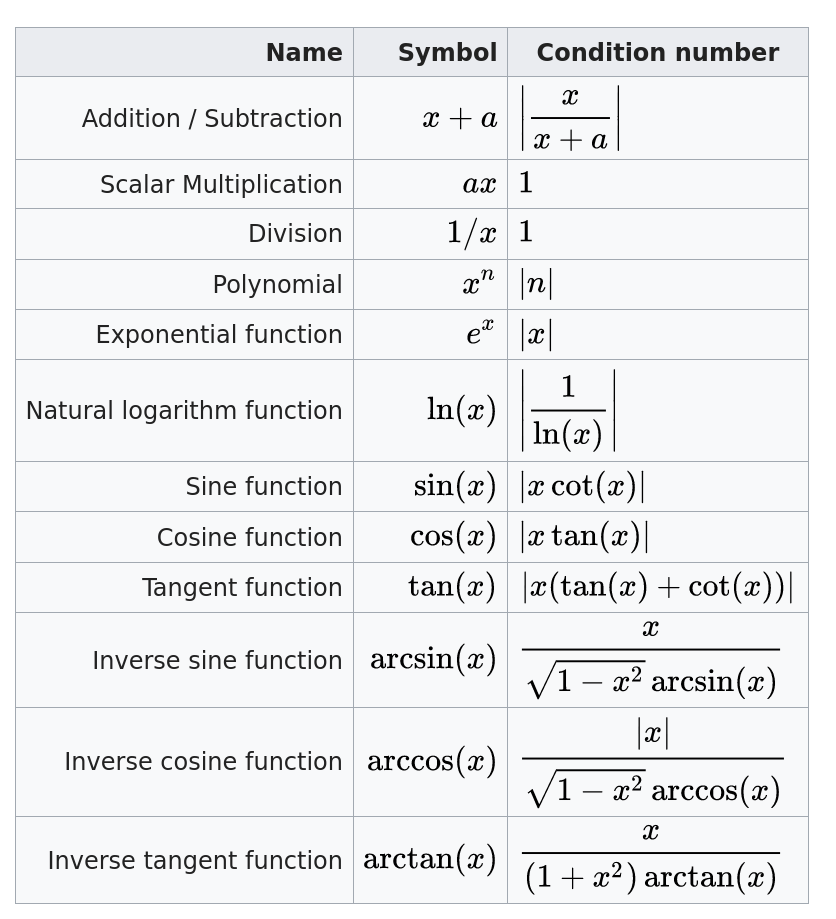
\includegraphics[width=0.5\linewidth]{basicOperations.png}
    \caption{Overview of relative condition number of basic operations.}
\end{figure}

Relative condition number of a multi-variant problem with one-dimensional output

\begin{equation}
    \kappa_{rel}(f, \vec{x}) =
    \frac{
        \sum_{i=1}^{n} \left| f_{x_i}(\vec{x}) \right| \cdot |x_i|
    } {
        \left| f(\vec{x}) \right|
    }
\end{equation}

Condition number of a matrix (e.g. choose the infinity matrix norm - row sum
norm)
\begin{equation}
    \kappa_{rel}(A) = ||A|| \cdot ||A^{-1}||
\end{equation}

Condition number of a single component of $\vec{f}(\vec{x}) : \mathbb{R}^n
\to \mathbb{R}^m$

\begin{equation}
    \kappa_{ij} = \frac{x_j}{f_i(\vec{x})} \pdv{f_i(\vec{x})}{x_j}
\end{equation}

\subsection{Loss of significant digits}

\begin{equation}
    \text{loss} = log_{10}(\kappa_{rel})
\end{equation}

\subsection{Rounding errors in floating point numbers}

Absolute rounding error
\begin{equation}
    |fl(r) - r| \leq 0.5 \cdot B^E
\end{equation}

Relative rounding error
\begin{equation}
    \left| \frac{fl(r) - r}{r} \right| \leq \frac{1}{2|M|} \leq \frac{B}{2}
    B^{-t}, \quad \text{because} |M| \geq B^{t-1}
\end{equation}

\subsection{Machine Precision}

Defined $\epsilon_0 := \epsilon_t := B^{1-t}$

Then we get an estimate on the rounded value
\begin{equation}
    fl(r) = r \cdot (1 + \epsilon), \quad |\epsilon| \leq \frac{\epsilon_0}{2}
\end{equation}

For the correct rounding we need $t+2$ digits on the computer, if the result has
to be accurate to $t$ digits.

\subsection{Unique solution to a perturbed linear system}

Only guaranteed if the absolute error is bounded
\begin{equation}
    ||\delta \mathbf{A} || < \frac{1}{||\mathbf{A}^{-1}||}
\end{equation}

\subsection{Forward stability}
Algorithm is forward stable if it introduces errors that are in a similar order
of magnitude as the unavoidable error due to the condition number. If the
algorithm consists of sub-algorithms the following estimate holds:
\begin{equation}
    \sigma_f \kappa_{rel}(f, x) \leq \sigma_g \kappa_{rel}(g, h(x)) + \sigma_h
    \kappa_{rel}(g, h(x)) \kappa_{rel}(h, x)
\end{equation}

\subsection{Backward Stability}
Set the disturbed output of our imperfect algorithm subject to unperturbed input
to be the output of a perfect algorithm of perturbed input data.
\begin{equation}
    \tilde{f}(x) = \hat{y} \quad \to \quad f(\hat{x}) = y
\end{equation}
If one can find an expression for $\hat{x}$ (i.e. how a perfect algorithm would
map this perturbed data to the correct output), this can be uses as a stability
estimator. If the backward error is bounded in a similar order of magnitude as
the condition the algorithm is called backward stable.

Backwards stability is a stronger attribute but more difficult to analyze. If an
algorithm is backward stable, it is also forward stable. The reverse is not
necessarily true.

%--------------------

\section{Matrix Factorization}

QR decomposition is unique aside from a sign.
LU decomposition is not unique and hardly depends on the pivoting strategy.

\subsection{LU Decomposition with Gauss-Jordan/Dolittle Algorithm}

Influence of Pivoting:

\subsection{QR Decompostion with Householder transformations}

Choose a vector by

\begin{equation}
    \vec{u} = A[i:, i] + sign(A[i,i]) \cdot norm(A[i:, i]) \cdot \vec{e}_1
\end{equation}


Householder transformations are unitary and hermitian.

\begin{equation}
    \mathbf{T}^{-1} = \mathbf{T}^H = \mathbf{T} = I_n - 2
    \frac{\vec{u}\vec{u}^H}{\vec{u}^H\vec{u}} \in \mathbb{C}^{n x n}
\end{equation}

\subsection{QR Decomposition with Givens Rotations}

Givens rotations are orthogonal and independent on the sign of the
rotation $\mathbf{R}(i,j,\phi)^{-1} = \mathbf{R}(i,j, -\phi) = \mathbf{R}(i,j,
\phi)^{T}$. They differ only in 4 elements from the identity matrix
$\mathbf{I}_n$. Assume you want to rotate the $a_{ij}$ element of matrix
$\mathbf{A}$ to zero. Then:

\begin{equation}
    r = sgn(a_{jj}) \sqrt{a_{jj}^2 + a_{ij}^2}
\end{equation}

Whereas $a_{jj}$ is the diagonal element in the column where we want to rotate
the element and $a_{ij}$ is the element we want to rotate to zero. Then we get
the values of cosine and sine (They never have to be calculated explicitly!)

\begin{equation}
    c = \frac{a_{jj}}{r}
\end{equation}

\begin{equation}
    s = \frac{a_{ij}}{r}
\end{equation}

Then the Givens rotation matrix is defined as follows:

\begin{equation}
    \mathbf{G}(i, j) = \mathbf{I}_n, \text{with} \quad
    G_{jj} = G_{ii} = c, \quad G_{ij} = -s = -G_{ji}
\end{equation}

To remember: The negative sine is always on a similar position as the element we
want to rotate.


If applied to get a $\mathbf{QR}$ decomposition eleminate the non-zero entries
below the main-diagonal by going columnwise from left to right and within the
columns from bottom to top.

\subsection{Cost of Decompositions}

\begin{itemize}
    \item $\mathbf{LU} \propto 2\frac{n^3}{3}$
    \item Householder $\mathbf{QR} \propto 4\frac{n^3}{3}$
    \item Givens $\mathbf{QR} \propto 6\frac{n^3}{3}$

\end{itemize}

\section{Polynomial Interpolation}

Polynomial Interpolation is unique because the the determinant of the
Vandermonde matrix

\begin{equation}
    \det \begin{pmatrix}
        1 & \dots & t_0^n \\
        \hdots & & \hdots \\
        1 & \dots t_n^n
        \end{pmatrix}
    =
    \prod_{i=0}^n \prod{j=i+1}^n (t_j -t_i)
\end{equation}

is non-zero if nodes are distinct. If not additional information on the
derivative has to be given.

\subsection{Lagrangian Form}

Calculate the Lagrange Polynomials on the interpolation nodes and then the
interpolating polynomial is given by

\begin{equation}
    P_n(t) = \sum_{k=0}^n y_k L_k(t)
\end{equation}

\subsection{Direct - Barycentric Lagrange Interpolation}

Rewrite the Lagrange Polynomial

\begin{equation}
    L_k(t) = \omega_{n+1}(t) \frac{w_k}{t-t_k}
\end{equation}

With the nodal polynomial of degree $n+1$

\begin{equation}
    \omega_{n+1}(t) := \prod_{i=0}^n (t - t_i)
\end{equation}

Then the weights can be precomputed

\begin{equation}
    w_k := \frac{1}{\prod_{k\neq j} (t_k - t_j}
\end{equation}

And the interpolating polynomial is given by

\begin{equation}
    P(t) = \omega_{n+1}(t) \sum_{k=0}^n \frac{w_k}{t-t_k} y_k
\end{equation}

Better stability properties than regular Lagrangian interpolation.

\subsection{Recursive - Aitken-Neville Algorithm}

Polynomial interpolation with Aitken-Neville of a set of $n+1$ data points to
interpolate a polynomial of degree $n$ in the form $P(x) = p_{0,n}(x)$. Start by
setting the initial values in the recursive scheme to $p_{i,i}(x)=y_i$. Then
calculate the other values by:
\begin{equation}
    p_{i,j}(x) = \frac{(x-x_j)p_{i,j-1}(x) - (x-x_i)p_{i+1,j}(x)}{x_i - x_j}
\end{equation}

More efficient evaluation of the Aitken-Polynomial at one certain point
\begin{equation}
    see matlab
\end{equation}

Aitken's theorem states that if two polynomial functions $M(t)$ and $N(t)$
interpolate $n-2$ common points, and $M(t)$ is additionally interpolating a
point before all the others and $N(t)$ is addtionally interpolating a point at
the end of the interval, then there is a unique polynomial $P(t)$ that
interpolates all value pairs as follows
\begin{equation}
    P(t) = N(t) + \frac{t - t_k}{t_k - t_i} (N(t) - M(t))
\end{equation}

\subsection{Recursive - Newton Algorithm}

Newton's Method provides a nice evalutation of a polynomial interpolation at
many points since it easily gives you the functional form of the interpolating
polynomial. Define the divided differences

\begin{equation}
    f[t_i, t_{i+1}, ..., t_k] =
    \frac{f[t_{i+1}, ..., t_k] - f[t_i, ..., t_{k-1}]}{t_k - t_i},
    \quad
    f[t_i] := f(t_i) = y_i
\end{equation}

Then the polynomial is defined as
\begin{equation}
    P(t) = \sum_{k=0}^{n} f[t_0, ..., t_k] \prod_{i=0}^{k-1}(t - t_i)
\end{equation}

If a derivative is given instead of a point, or an abscissa appears double and
it therefore has to be given the first derivative. The Newton's divided
difference becomes accurate to

\begin{equation}
    f[x_0, \dots, x_k] = \frac{f^{(k)}(x^*)}{k!}, \quad \text{if} x^* := x_0 =
    \dots = x_k
\end{equation}

Mind the $k!$ in the denominator (relevant for $k \geq 2$).

If the distance between points is equal (e.g. on an equidistant measurement
grid) we get

\begin{equation}
    f[x_0, \dots, x_k] = todo, see wikipedia
\end{equation}

\subsection{Horner's scheme for efficient evaluation}

Using Horner's scheme, the polynomial can be evaluated more efficiently
\begin{verbatim}
    P_n := f[t_0, t_1, ..., t_n]
    k=n-1:-1:0:
        P_k := P_{k+1} * (t - t_k) + f[t_0, t_1, ..., t_k]
\end{verbatim}

\subsection{Error in Polynomial Interpolation}

Compare the maximum componentwise error in approximation

\begin{equation}
    ||P_1 - P_2||_{\infty} = \left|\left| \sum_{k=0}^n y_k L_k - \sum_{k_0}^n
    \tilde{y}_k K_k \right|\right| =
    \leq \max_{k=0 \dots n} | y_k - \tilde{y}_k| \cdot \max_{t \in [t_0, t_n]}
    \left| \sum_{k=0}^n L_k(t) \right|
\end{equation}

The one can identify the Lebesguq constant for the lower bound of the error on
equidistant grids

\begin{equation}
    \Lambda(n) := \max_{t \in [t_0, t_n]} \sum_{k=0}^n L_k(t)
    \sim \frac{2^{n+1}}{n \ln(n)}
\end{equation}

This can lead to a definition of the conditioning for interpolation tasks on
equidistant grids.

For Chebychev grids these values increase way slower.

That means the choice of node placements has an important influence on the
accuracy of our interpolation. Assume $Q_n$ is the best interpolating
polynomial (best choice of node placement) and $P_n$ is our interpolating
polynomial (e.g. equidistant nodes). Then

\begin{equation}
    ||f - P_n||_{\infty} \leq (1 + \Lambda(n)) \cdot ||f - Q_n||_{\infty}
\end{equation}


\subsection{Chebychev nodal support for converging interpolation}

Chebychev nodes on an interval from $(a,b)$. $n$ nodes with index $k$. They are
the roots of the Chebychev polynomial of degree n.
\begin{equation}
    x_k = \frac{1}{2}(a+b) + \frac{1}{2}(b-a)\cos(\frac{2k-1}{2n}\pi)
\end{equation}

\subsection{Cubic Splines}

For efficient evaluation of cubic splines, use a different basis instead of the
standard monomial one (where we would have to solve for all 4 coefficients on
each sub-interval) - This basis has no special name
\begin{equation}
    \Pi_3 = \text{span}\left\{
        1 - \xi,
        \xi,
        -\frac{\xi}{3}+\frac{\xi^2}{2}-\frac{\xi^3}{6},
        -\frac{\xi}{6} + \frac{\xi^3}{6}
    \right\}, \quad \xi = \frac{t-t_i}{t_{i+1} - t_i}
\end{equation}

Then the interpolating polynomial is given by

\begin{equation}
    s_3(t) = y_i(1-\xi) + y_{i+1}\xi + h_i^2 y_i^{''} \left( -\frac{\xi}{3} +
    \frac{\xi^2}{2} - \frac{\xi^3}{6} \right) + h_i^2 y_{i+1}^{''} \left(
    -\frac{\xi}{6} + \frac{\xi^3}{6} \right)
\end{equation}

This is beneficial since $y_i$ is already available due to the inerpolating
condition. The second derivatives at each node can be efficiently computed.
Introduce the following abbreviations ($\mu_i + \lambda_i =1$)

\begin{equation}
    \mu_i := \frac{h_{i-1}}{h_{i-1} + h_i} = \frac{t_i -t_{i-i}}{t_{i+1} -
    t_{i-1}} > 0
\end{equation}
\begin{equation}
    \lambda_i := \frac{h_i}{h_{i-1} + h_i} = \frac{t_{i+1} - t_i}{t_{i+1} -
    t_{i-1}} > 0
\end{equation}

Then the following triagonal (non-square since we have 2 DoF) system has to be
solved

\begin{equation}
    \mu_i y_{i-1}^{''} + 2y_i^{''} + \lambda_i y_{i+1}^{''} = 6 y_{i-1,i,i+1}
\end{equation}

This creates $(n-2) x n$ system for the $n-2$ interior nodes. It uses the second
devided difference (refer to Newton's interpolation scheme) defined by

\begin{equation}
    y_{i-1,i,i+1} = \frac{y_{i,i+1} - y_{i-1,i}}{h_{i-1} + h_i}
\end{equation}

With the regular divided differenc given by

\begin{equation}
    y_{i, i+1} = \frac{y_{i+1} - y_i}{h_{i}}
\end{equation}

This system is underconstrained. We have to prescribe boundary conditions. These
can be of following type

\begin{itemize}
    \item Hermite splines $s_3^{'}(t_0) = y_0^{'}$ and $s_3^{'}(t_n) = y_n^{'}$ are
        prescribed
    \item $s_3^{''}(t_0) = y_0^{''}$ and $s_3^{''}(t_n) = y_n^{''}$ are
        prescribed. "Natural Spline" if both are set to zero.
    \item Periodic Splines $s_3^{'}(t_0) = s_3^{'}(t_n)$ and $s_3^{''}(t_0) =
        s_3^{''}(t_n)$ are prescribed
\end{itemize}

By the help of the Gershgorin Disks we can proof that under a given bounary
condition the cubic spline is unique.

Since we require the function to be interpolated to be $f \in \mathit{C}^4$ we
can define two upper bounds.

\begin{equation}
    L := \max_{t \in [a,b]} | f''''(t)|
\end{equation}

\begin{equation}
    H := \max_{0 \leq i \leq n-1} h_i
\end{equation}

Then upper bounds for the error on each subinterval can defined to

\begin{equation}
    |f - s_3| \leq \frac{7}{64} L \cdot H^2 \cdot h_i^2
\end{equation}
\begin{equation}
    |f' - s_3'| \leq \frac{7}{16} L \cdot H^2 \cdot h_i
\end{equation}
\begin{equation}
    |f'' - s_3''| \leq \frac{7}{8} L \cdot H^2 
\end{equation}
\begin{equation}
    |f''' - s_3'''| \leq 2 \cdot L \cdot H^2 / h_i
\end{equation}

By this we can conclude that that the splines converge against the function they
are interpolating for increasingly finer subintervals. For Polynomials this is
not given (only on Chebychev nodes).

\subsection{Cost of interpolation}

\begin{itemize}
    \item Lagrangian interpolation, each evaluation $O(n^2)$ additions and
        multiplications, adding new pairs requires completely new calculation.
        Computation can becom numerically unstable
    \item Barycentric Lagrange: Computing weights $\propto n^2$, adding value
        $\propto n$, evaluating polynomial $\propto n$
    \item Aitken-Neville : Storage only needs $n+1$ dimensional vector
    \item Newton: todo
    \item Cubic Splines in alternative form: Calculate the second divided
        differences, calculate parameters $\lambda_i$ and $\mu_i$, then solve
        tridiagonal system (can be accomplished by Thomas Algorithm $\sim O(n)$)
\end{itemize}


%%% ------
\section{Trigonometric Interpolation}

Instead of Polynomial interpolation trigonometric interpolation uses periodic
functions (e.g. $\sin(x)$ and $\cos(x)$ or $e^{ix}$ in general) to interpolate a
function on an interal $[a, b]$. The interpolation conditions holds and for the
actual task one has not to provide a function value for $b$ (i.e. $f(b)$)
because the function is assumed to be periodic on this interval, so $f(a) =
f(b)$.

A special case is the trigonometric interpolation with an equidistant spacing
between the interpolating points on the basic periodic interval $[0, 2\pi]$:

\begin{equation}
    x_k = \frac{k\cdot 2 \cdot \pi}{n}, \quad \text{with} \; k=0, 1, \dots, n-1
\end{equation}

Every other interval can be transformed to this interval by a linear
transformation.

The trigonometric functions make up the basis of the $L_2$ space, i.e.

\begin{equation}
    L_2 = span \{e^{jx} \}, \quad \text{with} \; j \in \mathbb{Z}
\end{equation}

One is basically free to choose the $n$ functions to interpolate the values
with. However, similar to polynomial interpolation choosing only the lowest
degree ones (in terms of trigonometric interpolation the ones with the lowest
frequencies) one minimizes the interpolating error. Additionally the
interpolating coefficients coincide with the values of the discrete Fourier
Transform.

\subsection{Continous Fourier Transform}

Find the coefficients by 

\begin{equation}
    c_k := \frac{1}{2\pi} \int_0^{2\pi} f(x) e^{-ikx} \; \mathrm{d} x, \quad k
    \in \mathbb{Z}
\end{equation}

Get the Fourier series of f by

\begin{equation}
    S_f(x) = f(x) = \sum_{-\infty}^{\infty}c_k e^{ikx}
\end{equation}

\subsection{Discrete Fourier Transform (DFT)}

Discrete Function values are given on equidistant abscissae on $(0, 2\pi)$
exluding the right boundary of the interval.

The coeffients of the interpolation (these are approximations of the Fourier
coefficients of the $n$ lowest frequencies) are found by solving the system

\begin{equation}
    \sum_{j=\lceil -n/2 \rceil}^{\lceil n/2 \rceil} \gamma_j e^{i\cdot j \cdot x_k} = y_k
\end{equation}

Or in matrix vector notation
\begin{equation}
    \mathbf{F} \vec{\gamma} = \vec{y}, \quad \text{with} \; F_{kj} = e^{i\cdot
    \frac{2\pi}{n} \cdot jk}
\end{equation}

The matrix $\mathbf{F}$ is perfectly conditioned and almost unitary
$\mathbf{F}^{-1} = \frac{1}{n} \mathbf{F}^H$. Therefore, in this very special
case the system can be solved by using the inverse.

The one can assemble the approximate Fourier Series to

\begin{equation}
    f(x) \approx T_n(x) = \sum_{j=\lceil -n/2 \rceil}^{\lceil n/2 \rceil} \gamma_j e^{i\cdot j}
\end{equation}

Remarks:
\begin{itemize}
    \item When interpolating real values, it holds $\gamma_k =
        \bar{\gamma_{-k}}$
    \item When interpolating real values, the interpolating polynomial is also
        real (transform to it via Euler's Identity)
\end{itemize}

In case of $n$ being even (this means an uneven distribution of the lowest
frequncies around $0$), it is arbitrary whether if one chooses $\lceil -n/2
\rceil$ or $\lceil n/2 \rceil$. Since this is not allowed to have an influence
on the solution, the contribution by this frequency may only be real.

\subsection{Fast Fourier Transform (FFT)}

Performing the DFT takes $O(n^2)$ operations. This can be reduced by exploiting
the shape of the matrix. By the help of permuations one can subdivide the matrix
$\mathbf{F}$ into matrices of half sice, reducing the effort to $O(n\log(n))$
with the fastest result if $n$ is a power of $2$.


%%% --------------------
\section{Quadrature - Numerical Integration}

\subsection{Newton-Cotes-Methods}

Newton-Cotes type quadrature interpolates the integrand by the help of
polynomials on an equidistant grid. Composite rules define their sub-interval
length to $\frac{b-a}{n}$ with n sub-intervals.


\begin{table}[H]
    \centering
    \begin{tabulary}{\linewidth}{C C C}
        \toprule
        name & definition & remainder\\
        \midrule
        Trapezoid &
            $\displaystyle \frac{b-a}{2} (f(a) + f(b)) $ &
            $\displaystyle -\frac{f^{''}(\eta)}{12}(b-a)^3$
        \\
        Kepler &
            $\displaystyle \frac{b-a}{6} \left( f(a) + 4f(\frac{a+b}{2}) + f(b)
            \right)$ &
            $\displaystyle - \frac{f^{(4)}(\eta)}{90} \left(\frac{b-a}{2}
            \right)^5$
        \\
        \midrule
        Comp. Trapez. &
            $\displaystyle \frac{h}{2} \left( f(a) + 2 \sum_{j=1}^{n-1}f(x_j) +
            f(b) \right) $ &
            $\displaystyle - \frac{b-a}{12} h^2 f^{''}(\eta)$
        \\
        Simpson &
            $\displaystyle \frac{h}{3} \sum_{j=1}^{n/2} \left[ f(x_{2j-2}) + 4
            f(x_{2j-1}) + f(x_{2j}) \right] $ &
            $\displaystyle - \frac{h^4}{180}(b-a) f^{(4)}(\eta)$
        \\

        \bottomrule

    \end{tabulary}
\end{table}

\subsection{Adaptive Composite Rules}

\begin{itemize}
    \item Start with course sub-intervals $h_1$
    \item Half the sub-interval-lengths everywhere $h_2=h_1/2$
    \item For each interval calculate the error $err_j = |S_{\text{coarse}} -
        S_{\text{fine}}|$
    \item Weight each error with the sub-interval length $err_j \frac{h_j}{b-a}$
    \item Refine the sub-intervals further (recursively) if error is above a set
        tolerance
\end{itemize}

\subsection{Romberg's Extrapolation Method}
Let $T(h)$ denote the composite trapezoidal approximation of an integral with
$n$ subintervals each of length $h$. Then the error according to
\emph{Euler-Maclaurin} reads
\begin{equation}
    R(h) = \sum_{k=1}^{n+1} b_{2k}(0)h^{2k} \cdot f^{(2k -1)}(x)
    \bigg|_{x=a}^{x=b} - h^{2n+2} \int_a^b b_{2n+2}(\frac{x-x_i}{h})
    f^{(2n+2)}(x) \, \mathrm{d} x
\end{equation}

According to this the error expands in $h^2$. 

\begin{equation}
    R(h) = c_1 h^2 + c_2 h^4 + c_3 h^6 + \dots + c_m h^{2m} +
    \alpha_{m+1}(h)h^{2m+2}
\end{equation}

We know that we have the true
solution of the integral for an infinitely small sub-interval width $h$.
Therefore, we can expand the function $T(h)$ in terms of $h^2$ and make an
extrapolation at $h=0$.

Then, with the help of the Aitken-Algorithmi ($R_{i,i} = T(h_i)$), Romberg's
method reads
\begin{equation}
    R_{i,k} = \frac{h_k^2}{h_k^2 - h_i^2}R_{i, k-1} - \frac{h_i^2}{h_k^2 -
    h_i^2} r_{i+1, k}
\end{equation}

In the case of the Romberg sequence of sub-interval length (halfing each time),
we get
\begin{equation}
    R_{i, k} = \frac{4^{-k}}{4^{-k} - 4^{-i}} R_{i, k-1} - \frac{4^{-i}}{4^{-k}
    - 4^{-i}} R_{i+1, k}
\end{equation}

The error estimator is given as
\begin{equation}
    R_n = O(\prod_{i=0}^{n-1} h_i^2)
\end{equation}

One can derive the Trapezoidal-Rule and the 3/8 Rule with the help of Romberg
but with a worse error estimator.

Mind that Richardson's idea is not applicable to periodic functions integrated
over one period, since the error expansion term vanish. Outcome: split up
quadrature interval into two !unequally long intervals! and apply Romberg on
them.

\subsection{Gauss-Legendre Quadrature}


%%% --------------
\section{Eigenvalues}

Eigenvalues should numerically never be determined by the roots of the
characteristic polynomial. Instead use other algorithms like (inverse) power
iteration or the QR algorithm. Then the condition number of finding an
eigenvalue is given as

\begin{equation}
    \kappa(\lambda) = ||\mathbf{V}||\cdot||\mathbf{V}^{-1}||
\end{equation}
With the eigenvector matrix $\mathbf{V}$. If the matrix $\mathbf{A}$ is normal,
i.e. $\mathbf{AA}^H = \mathbf{A}^H \mathbf{A}$, then $\mathbf{V}$ is unitary and
the problem is perfectly conditioned.

\subsection{Power Iteration}

Choose an arbitrary vector $\vec{q}_0$. Then perform one iteration

\begin{equation}
    \vec{q}_{i+1} = \vec{q}_i^H \mathbf{A} \vec{q}_i
\end{equation}

Normalization ensures that no overflow occurs.
The approximation to the biggest eigenvalue is given by the Rayleigh Quotient

\begin{equation}
    \mu_i = \frac{\vec{q}_i^H \mathbf{A} \vec{q}_i}{\vec{q}_i^H \vec{q}_i}
\end{equation}

Converges against the greatest eigenvalue. $\vec{q}$ is a bad approximation of
the corresponding eigenvector.

Converging if, greatest eigenvalue is distinct or appears multiple times. 
If greatest eigenvalue also has its negative or is the complex conjugate, no
convergence.
Convergence is faster, the smaller the ratio $|\lambda_i/\lambda_1|$.

Define residual
\begin{equation}
    \vec{r}_i = \mathbf{A}\vec{q}_i - \mu_i \vec{q}_i
\end{equation}

Stopping criterion
\begin{equation}
    \frac{||\vec{r}_i||}{|\mu_i| \cdot ||\vec{q}_i||} \leq \sigma \epsilon_0
\end{equation}

\subsection{Inverse Power Iteration}

Choose arbitrary vector $\vec{q}_0$ and initial guess $\sigma_0$ (for example by
one step of a regualr power iteration.

Then perform one iteration
\begin{equation}
    (\mathbf{A} - \mu \mathbf{I})\vec{q}_{i} = \vec{q}_{i-1}
\end{equation}

Approximation to the eigenvalue is given by the Rayleigh Quotient. Converges
against eigenvalue closest to guess $\mu$. $\vec{q}$ converges quite well
against the corresponding eigenvector.

Costs $O(n^2)$ flop per step when LU decomposition of shifted matrix is saved.

\subsection{QR Algorithm}

First preconditioning, transform general matrix into upper Hessenberg form or
Hermitian matrix into real! tridiagonal form by QR modifications:
\begin{enumerate}
    \item Choose a first column and get an Householder so that all entries below
        the subdiagonal would be zero
    \item Apply $A \to T^{-1}AT$
\end{enumerate}

Then iterator over the following algorithm
\begin{enumerate}
    \item $Q_k R_k = R_{k-1}\quad$ Decompose into QR of a previous
    \item $T_k := R_k Q_k \quad$ Reverse order of multiplication 
\end{enumerate}


\subsection{Shifts}

For QR-Algorithm. 
\begin{enumerate}
    \item $Q_k R_k = R_{k-1} - \mu I \quad$ Decompose into QR of a previous
        matrix minus shift
    \item $T_k := R_k Q_k + \mu I \quad$ Reverse order of multiplication and add
        the shift
\end{enumerate}

\subsection{Rayleigh Shift}

Use bottom right element as shift. Once element in subdiagonal in last row is
close to zero, deflate the rest of the matrix.

Does not work for complex EWs. 

\subsection{Wilkinson Shift}

Consider the matrix 2x2 block in the bottom right. Analytically calculate the
eigenvalues and use this eigenvalue as a shift that is the closest to the bottom
right element

%%%--------------------
\section{Nonlinear Equations}

\subsection{General}
Derivation: Take Taylor Series up to constant or linear term and approximate the
derivatives.

General form:

\begin{equation}
    x^{[n+1]} = x^{[n]} - \frac{f(x^{[n]}}{q^{[n]}}
\end{equation}

Whereas the basic methods only differ in their choice or approximation of
$q^{[n]}$

\subsection{Chord Method}

\begin{equation}
    q_k = \frac{f(b) - f(a)}{b - a} = const
\end{equation}

Onstep method, converges with $p=1$

\subsection{Secant Method}

\begin{equation}
    q_k = \frac{f(x_k) - f(x_{k-1})}{x_k - x_{k-1}}
\end{equation}

Two-Step Method, converges locally with $p \approx 1.63$.

\subsection{Regula Falsi - False Positive}

Choose the two pairs of the values so that at least one zero of the function is
between the secant.

Same computational effort as Secant Method but globally convergent with $p=1$

\subsection{Anderson-Björck}

Modification of Regula Falsi, provides an "adaptive" mix between it and secant
method

In case of simple roots, superlinear and globally converging with $p \approx
1.7$

Method of Choice in 1D cases.

\subsection{Newton's Method}

\begin{equation}
    q_k = f'(x_k)
\end{equation}

Converges locally with $p=2$ for single roots and with $p=2$ for multiple roots.

\subsection{Simplified Newton}

Derivative is calculated once ($p=1$) or recalculated after $n$ iteration steps.

\subsection{Bisection Method}

Consecutively half the search interval (divide and conquer approach) and choose
that interval in which the sign of the function changes (indicates the root is
in that interval).

Simple, extremely stable and globlly convergent (worse than linear)

Method of choice for multple roots, e.g. rough estimate by Newton or
Anderson-Björck and then further refinement with Bisection.

\subsection{Fixed-Point Methods}

The presented iterative methods for root-finding form a subset of Fixed-Point
Methods (ODE Methods, Eigenvalue methods etc. can also be categorized in this
regard, but difficult to analyze).

Fixed point defined

\begin{equation}
    \lim_{k \to \infty} x_k = x^*, \quad \Phi(x^*) = x^*
\end{equation}

The Method is called contractive if it reduces the distance between two points
in the subset it operates on

\begin{equation}
    |\Phi(x) - \Phi(y) | \leq L \cdot | x - y |, \quad \forall x, y \in [a, b]
\end{equation}

With a Lipschitz-Constant that has to be $L<1$ for convergence.

If the the iteration $\Phi(x)$ is differentiable (!!! Important, no analysis for
non-differential functions possible, errors not bounded), then

\begin{equation}
    L \geq \left| \frac{\Phi(x) - \Phi(y)}{x - y} \right| = \Phi'(z), \quad
    \forall z \in [a,b]
\end{equation}

\subsection{Order of Convergence for Contractive Fixed-Point Methods}

$\Phi$ converges (locally) to $x^*$ with order $p \geq 1 $, if for $\epsilon > 0
$ properly chosen

\begin{equation}
    \exists C > 0 : |\Phi(x) - x^*| \leq C |x - x^*|^p, \quad \forall x \in [x^*
    - \epsilon, x^* + \epsilon]
\end{equation}

and $C < 1$ in case of linear ($q = 1$).

In other words: The distance to the fixed-point has to be reduced for in every
iteration

!!! The order of convergence is equal to the order of the first non-vanishing
derivative of $\Phi$

\subsection{Fixed Point Theorem}

If (a) a fixed point method is confined to one interval and (b) contractive
\begin{equation}
    x_k \in [a, b], \quad \forall k=0,1,2, \dots
\end{equation}
\begin{equation}
    |\Phi(x) - \Phi(y)| \leq L \cdot |x - y|, \quad \forall x, y \in [a, b]
    \quad \text{with} L<1
\end{equation}

Then the following holds:
\begin{enumerate}
    \item The fixed point exists in the limit in the interval $[a, b]$
    \item it is the only fixed point in the interval
    \item the fixed point method converges at least linearly
\end{enumerate}

Additionally some insights on the distance to the fixed point,
\begin{equation}
    |x_k - x*| \leq L^k |x_0 - x*|
\end{equation}
\begin{equation}
    |x_k - x* | \leq \frac{L^k}{1-L}|x_0 - x_1|
\end{equation}

\end{document}
